\documentclass{article}

\usepackage[utf8]{inputenc}
\usepackage{graphicx}
\usepackage{float}
\usepackage{listings}
\lstset{
    frame=single,
    breaklines=true,
}

\begin{document}
\title{FYS1210 - Lab 5}
\author{Robin.A.T.Pedersen \and Dawid Patryk Kuleczko}
\maketitle

\section{Formål}
Oppgaven skal gi en innføring i digitale kretser.
\\\\
Vi skal se hvordan digitale kretser er bygget opp av komponenter.
Og hvordan egenskapene til disse bestemmer kretsens ytelse.
Det er også en øvelse i bruk av oscilloskop og signalgenerator,
med vekt på oscilloskopets \emph{cursor}-funksjon.
\\\\
Utgangspunktet er i en diode-transistor krets (DTL - diode transistor logikk).
Vi ser på en NAND-krets og skal se på de logiske og elektriske egenskapene.
Hva skjer når man legger til en Schottky-diode mellom collector og base på
en switch-transistor?
\\\\
Vi skal også undersøke egenskapene til en low-power-schottky NAND.


\section{Oppgave 1}
Kretsen vår er en NAND.
Det er to input, A og B, og en output Y.
Spenningen avgjør om signalet regnes som 1 eller 0.
\\\\
Et potmeter gjør at vi kan justere spenningen på A. \\
Input B er alltid 1, men en knapp setter den til 0. \\
En lysdiode, aktivert av strap S2, indikerer om output er 1 eller 0.

\subsection{Potmeter}
Hvor går spenningsgrensen mellom 1 og 0 i logikken?
\\
Hvis B alltid er på, og lampa av når begge er på, skrur vi A opp til lampa
er av.
Da kom vi opp til ~1.1 volt.
Det betyr at grense mellom 1 og 0 (i port-logikken) er ca 1.1V.

\subsection{Oppg 1}
Prøv forskjellige kombinasjonene av A og B og verifiser funksjonstabellen.
\\\\
\begin{tabular}{l|c|r}
  A & B & Y \\ \hline
  0 & 0 & 1 \\ \hline
  0 & 1 & 1 \\ \hline
  1 & 0 & 1 \\ \hline
  1 & 1 & 0 \\
\end{tabular}
\\\\
Strap S2 er på så vi kan observere om output er 1 eller 0.
Deretter vrir vi potmeteret for å justere A mellom 0 og 5 volt.
\begin{itemize}
\item Vi skrur A=0 og trykker ned B=0.
      Dioden lyser! Akkurat som forventet.
\item Fortsatt er A=0 og slipper opp B=1.
      Dioden lyser! Akkurat som forventet.
\item Vrir opp A=1 og trykker ned B=0.
      Dioden lyser! Akkurat som forventet.
\item Fortsatt er A=1 og slipper opp B=1.
      Det kommer en tid i enhver diodes liv hvor lyset tar slutt.
\end{itemize}


\section{Oppgave 2}
Vi fjerner strap S2.

\subsection{Oppg 2a}
La B være ’høy’ - (ikke trykk på knappen) \\
Ved hvilken spenning på A skifter utgangen tilstand til lav? Forklar hvorfor.
\\\\
Vi måler utgangsspenningen mens vi justerer spenningen over A fra 5V og nedover.
Utgangsspenningen holder seg på ca 21mV lenge til den såvidt begynner å stige.
Den stiger svakt i mV skala til den plutselig hopper opp til 1V.
Der er spenningen over A ~1.1V.

\paragraph{Forklaring} \mbox{} \\
For at det skal gå strøm gjennom transistoren må strømmen gjennom D3, D4 og BE,
tilsammen må spenningen være $0.6 + 0.6 + 0.6 = 1.8$.
Vi måtte spille A til 1.1V som sammen med dioden er $1.1 + 0.6 = 1.7$.
Fordi diodene ikke er perfekte vil det gå strøm litt før ideelt sett,
altså er 1.7 nok til å få strøm i kretsen.



\subsection{Oppg 2b}
Tegn opp sammenhengen mellom spenningen over A og 
Vut.  
Pass på å få med med noen ekstra verdier rundt overgangen 
fra ’høy’ til ’lav’.
\begin{figure}[!ht]
  \caption{Sammenheng mellom spenning over A og spenning ut.}
  \centering
    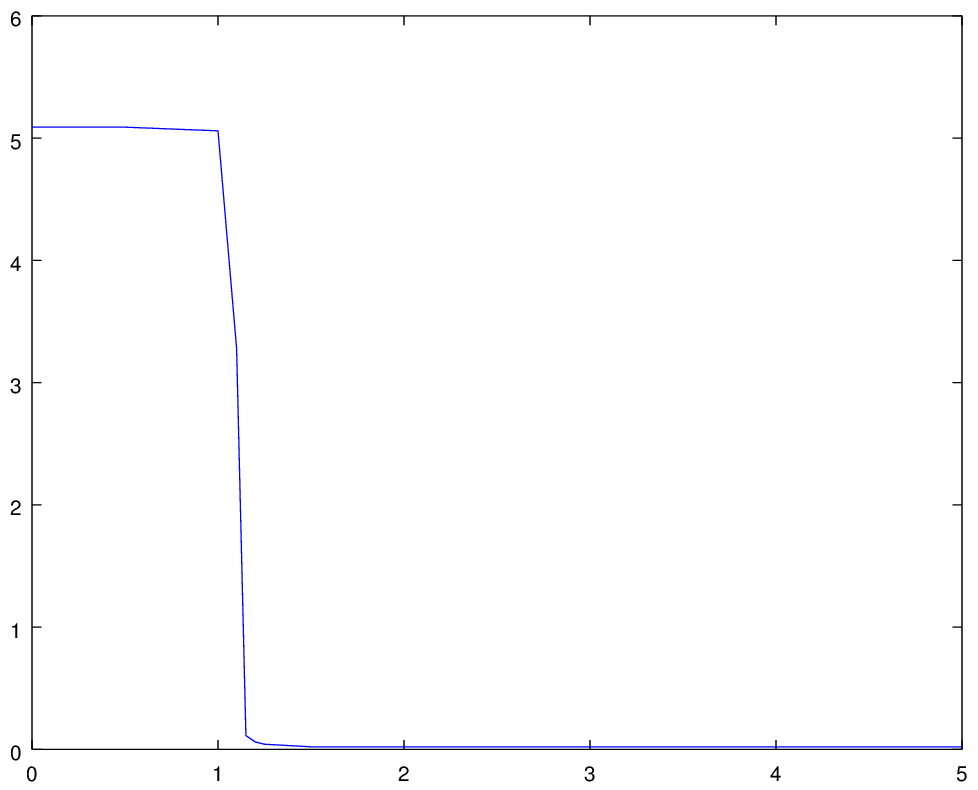
\includegraphics[width=\textwidth]{2b.png}
\end{figure}

\begin{figure}[!ht]
  \lstinputlisting{2b.matlab}
  \caption{Koden tilhørende plot.}
\end{figure}


\section{Oppgave 3}
På de neste oppgavene bruker vi funksjonsgeneratoren TG550 som signalkilde.
Vi stiller inn funksjonsgeneratoren og oscilloskopet slik det er
beskrevet i oppgaven.

\subsection{Oppg 3}
A settes til 5 volt.  
Inngangssignalet til B er en sinusspenning med frekvens 1 kHz og vi varier
signalamplituden (Vpp) fra 2 til 6 Vpp. 
Vi sammenligner inngangssignal og utgangssignal.
\\\\
For input Vpp fra 2V og oppover får vi utslag i output signalet.
Der hvor input signalet er over 2V får vi en negativ puls på output.
\begin{figure}[H]
  \caption{Sinusfunksjon på input B og output-signal.}
  \centering
    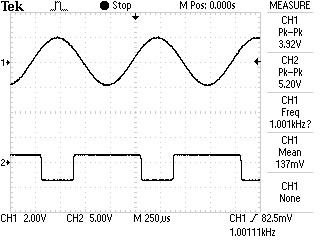
\includegraphics[width=\textwidth]{3.jpg}
\end{figure}


\section{Oppgave 4}
Flytt BNC-T leddet fra MAIN OUT til AUX OUT/TTL/CMOS.
Dette gir et firkantsignal (TTL-signal) som skifter mellom 0V og 5V.
Sett frekvensen til 1kHz.



\subsection{Oppg 4a}
Finn høyeste frekvens DTL-kretsen klarer å gjengi.
Det vil si frekvensen hvor ikke lenger utgangspulsene overstiger
halve inngangsspenningen.
\\\\
Vi justerte frekvensen opp til 150kHz hvor vi så at utgangspulsene var halveis
på inngangspulsen.
\begin{figure}[!ht]
  \caption{Høyeste gengivbare frekvens.}
  \centering
    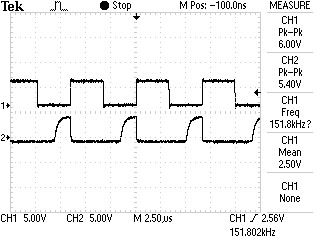
\includegraphics[width=\textwidth]{4a.jpg}
\end{figure}
Komponentene i kretsen bruker litt tid på å reagere.
Og på et tidspunkt vil inngangsfrekvensen være så hyppig at komponentene
ikke lenger rekker å reagere fort nok.



\subsection{Oppg 4b}
Vi stiller signalet til 100kHz og stiller inn cursoren.
Forsinkelsen før reaksjon er på 1,92us eller 1920ns.
\begin{figure}[!ht]
  \caption{Forsinkelse i kretsen.}
  \centering
    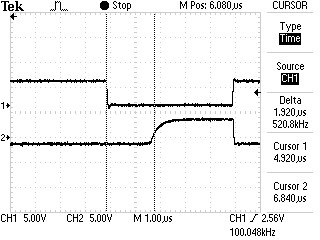
\includegraphics[width=\textwidth]{4b.jpg}
\end{figure}
Transistor opererer i metning og bruker tid på å gjenopprette
sperresjikte mellom base og collector.
\\\\
I motsatt retning retning er forsinkelsen \emph{mye} mindre.
Vi måler 28ns.
\begin{figure}[!ht]
  \caption{Forsinkelse i kretsen.}
  \centering
    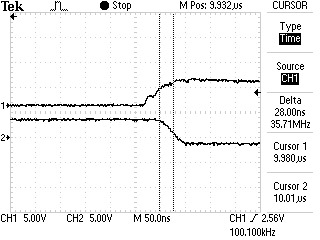
\includegraphics[width=\textwidth]{4bb.jpg}
\end{figure}


\section{Oppgave 5}
Vi setter input-frekvensen tilbake til 150kHz og kobler på schttky-dioden med
strap S1.
I oppgave 4a er bildet fra før dioden kobles inn.
\\\\
Med schottky-dioden kan man øke frekvensen betraktelig høyere.
Vi justerte opp til ca 1.2MHz.
\begin{figure}[H]
  \caption{Forsinkelse i kretsen med schottky-diode.}
  \centering
    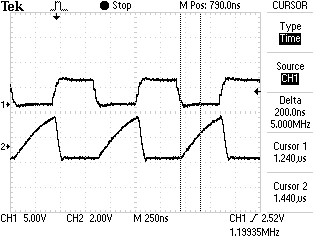
\includegraphics[width=\textwidth]{5.jpg}
\end{figure}
Schottky-dioden hindrer transistoren fra å gå i metning.
Da holder transistoren mindre ladningen og det går raskere å bytte modus.


\section{Oppgave 6}
\subsection{Oppg 6a}
Mål karakteristikker for en av kretsene i 74LS00.
Vi måler for kretsen \emph{med} strap S3 koblet til.
\\\\
Utgangsspenning som funksjon av inngangsspenning.
\begin{figure}[H]
  \caption{Forholdet mellom inngang- og utgangsspenning.}
  \centering
    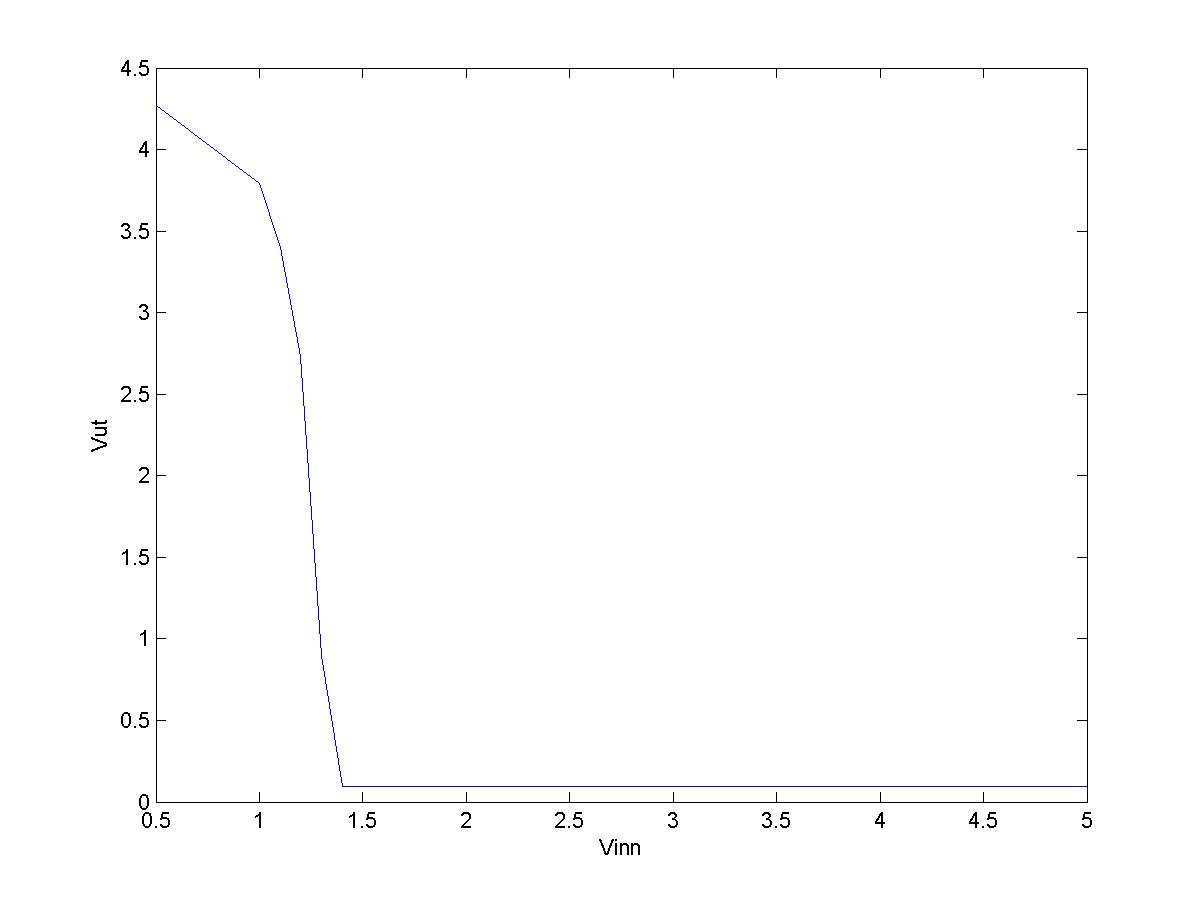
\includegraphics[width=\textwidth]{6a.jpg}
\end{figure}

Når vi skal måle strømmen er må vi regne ut spenningen over motstanden R5,
så vi kobler inn strap S3.
Vi måler spenningen over motstanden og regner ut strømmen basert på det, før vi
plotter det i forhold til inngangsmotstanden.

\begin{figure}[H]
  \caption{Forholdet mellom inngangstrøm og inngangsspenning.}
  \centering
    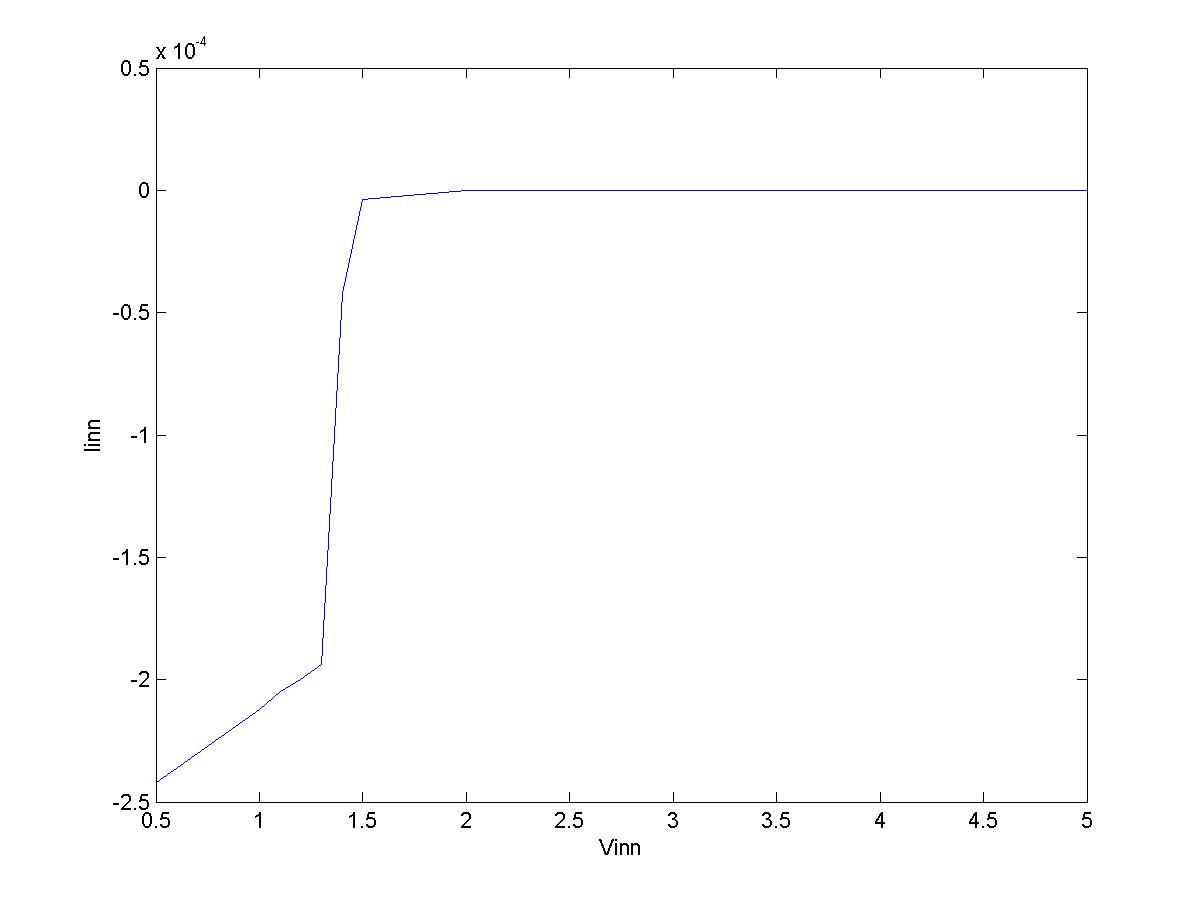
\includegraphics[width=\textwidth]{6aa.jpg}
\end{figure}



\subsection{Oppg 6a}
Vi setter frekvensen såpass høyt at vi ser utgangspulsens forsinkelse.
Når vi stiller inn cursor får vi en delta-tid på 33ns og en frekvens på 30MHz.
Det vil si at kretsen klarer å gjengi signaler på ~15MHz.
\begin{figure}[H]
  \caption{Forsinkelse i utgangspulsen.}
  \centering
    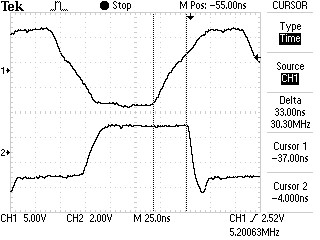
\includegraphics[width=\textwidth]{6b.jpg}
\end{figure}



\subsection{Oppg 6c}
TODO


\end{document}
